\begin{frame}
  \frametitle{Как да започнем ?}
  \begin{itemize}
      \item Упражнения, малък проект в къщи
      \item Изграждане на инфраструктура, на работа
      \item Measure code coverage
      \item bug report -> write test -> fix
      \item new features -> tdd
      \item write test -> refactor legacy code
  \end{itemize}
\end{frame}

\begin{frame}
  \frametitle{Заключение}
  \begin{itemize}
      \item Качеството е форма и фунцкия
      \item Test suite -> по-добра форма
      \item Test suite -> не губим фунцкия
      \item TDD -> Test suite
  \end{itemize}
\end{frame}

\vspace*{-12.5mm}    
\begin{frame}[fragile, plain]
\frametitle{}
\hspace*{-11mm}
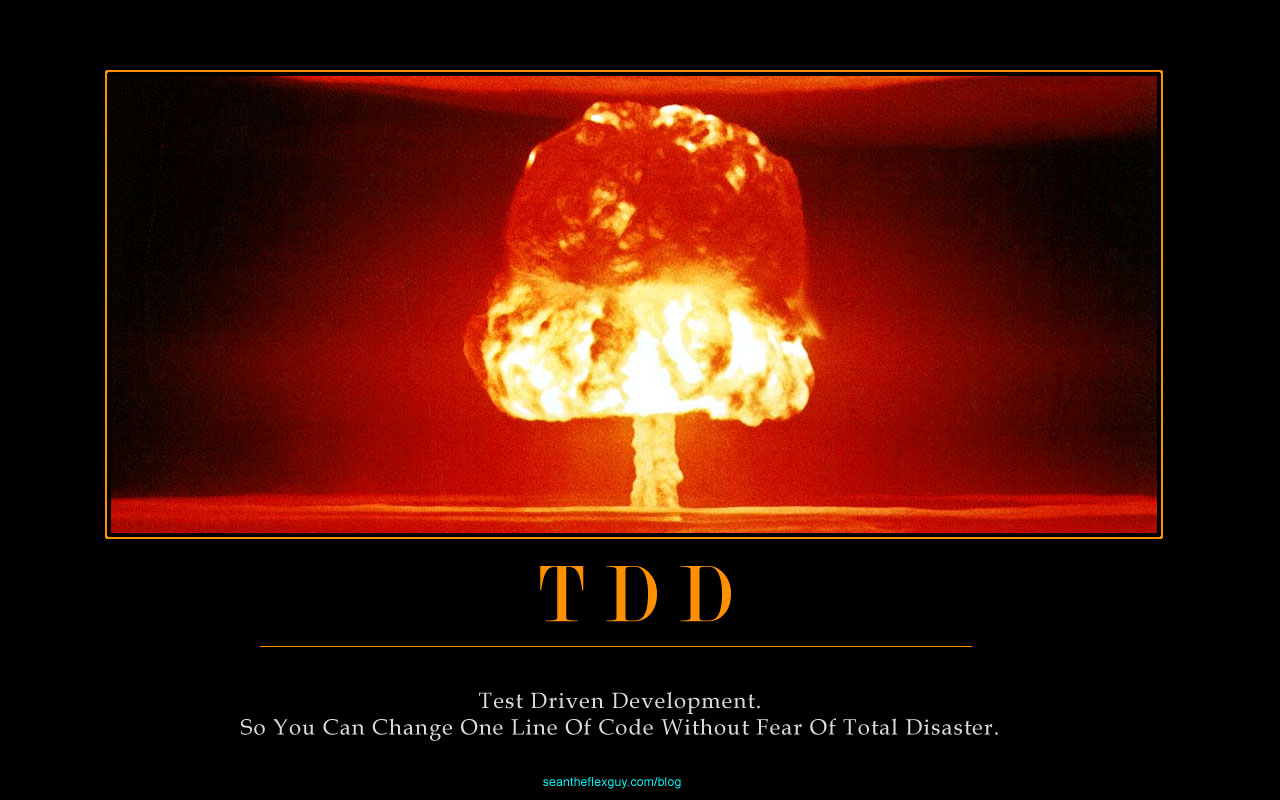
\includegraphics[width=\paperwidth, width=\paperwidth]{tdd.jpg}
\end{frame}

